\chapter{Indledning}

\section{Baggrund}
En normal synkeproces er kendetegnet ved at fødeindtagelse som passerer fra den bageste del af mundhulen, via. svælget og spiserøret til mavesækken sker uden besvær. Tilstanden hvori selve synkefunktionen og dens hastighed og frekvens forstyrres kaldes for dysfagi \cite{Sundhedsstyrelsen2015NationalDysfagi}. Dysfagi er den medicinske betegnelse for symptom relateret til synkebesvær. Der er vigtigt at differentiere mellem nedre og øvre dysfagi. Øvre dysfagi omfatter præ-oral, oral og faryngeal fase, hvorimod nedre dysfagi relaterer sig den øsefageale fase dvs. mavesæk og spiserør \cite{KjaersgaardPh.d.studerendeDYSFAGIKonsekvenser}. Det skal dog nævnes, at der er uenigheder om definitionen af dysfagi. Den manglende konsensus om definitionen gør rapportering af dysfagi insidens og prævalens uklar. Det fremgår af patientombuddets temarapport fra 2012 om dysfagi at:

\begin{itemize}
\item 60-87 \% af beboere på plejehjem for ældre har synkebesværligheder.
\item 30 \% alle apopleksipatienter har dysfagi. 15.000 danskere rammes hvert år af apopleksi. Forekomsten af dysfagi er ca. 37-78 \% ved akut apopleksi. Hos patienter med i den akutte fase, er dysfagi/aspiration en betydende årsag. Herudover lever 30-40.000 danskere med senfølger efter en apopleksi, nogle har dysfagi
\item 20-50 \% af patienter med Parkinson og Alzheimer har dysfagi. I 2012 havde 6. 000 patienter Parkinson og 45.000 patienter havde Alzheimer.  
\item 30-60 \% af patienter med muskelsvind har dysfagi.
\item Derudover er der ca. 10.000 børn, unge og voksne med Cerebral Parese (CP) eller kendt som "spastisk lammelse", der har synkebesvær \cite{Bommersholdt2012TemarapportDysfagi}. 
\end{itemize}

Som det ses i de nævnte statistikker, rammer dysfagi en bredt vifte af patienter fra forskellige patientgrupper. Årsagerne og konsekvenserne til dysfagi kanlæses i \nameref{bilag1}. 

Udredning af øvre dysfagi består af en diagnostisk strategi med tre trin: en tidligere screening, som skal afdække tilstedeværelsen af synkebesværligheder, en allround klinisk undersøgelse, der estimerer synkebesværlighedens omfang og en instrumentel undersøgelsesmetode vha. Fiber Endoskopisk Evaluering af Synkefunktionen (FEES) og/eller Funktionel Videoradiologisk Evaluering af Synkefunktionen (FVES). Alle nævnte undersøgelsesmetoder er manuel undersøgelser, der indeholder flere subjektive elementer som klinikeren rapportere undervejs i undersøgelsen og som kan forringe undersøgelsens kvalitet. Den ringe kvalitet kan give underdiagnostik og dermed dårlig tilrettelæggelse af et behandlingsforløb. I \nameref{bilag1} belyses hvordan FEES og FVES foretages. Begge metoder anvendes til at dømme aspirationsrisiko og til at angive anbefalinger for oral indtagelse, men flere studier viser at begge metoder ikke er tilstrækkelige pålidelige, dyre i pris og ofte ikke gentagelige \cite{Kelly2006} \cite{McCullough2001Inter-Measures} \cite{Schultheiss2014} \cite{Nahrstaedt2012SwallowMeasurements}.  Der er derfor brug for alternative metoder, som kan give objektiv detektion af synke problemer. En af disse metoder er at kombinere elektromyografi (EMG) og bioimpedans sensorer. Et forudgående projekt til dette projekt har anvendt prisvenlig EMG sensor af typen MyoWareTM Muscle Sensor til at måle synkesignaler på raske personer med succes \cite[s. 58]{ChristensenElisabethLundbakStrand2017} da den kun bidrager med informationer om muskel aktiviteten i de muskel, der deltager synkningen. Derfor anvender projektet en prisbillig bioimpedans sensor som en gruppe forskere har anbefalet og anvist til en opskrift til udvikling af en bioimpedansmåler \cite{Aroom2009}.

Bioimpedans er kompleks modstand, der kan anvendes til at måle den elektrisk impedans i vævet ved at udnytte forholdet mellem spænding og strøm. Ved væske, fødeindtagelse eller vejrtrækning ændres forholdet mellem spænding og strøm i svælget og det er denne ændring, der er indeholder informationer om 
synkefunktionens tilstand. Som det ses på figur \ref{EMGBIGraph}, er svælget åben og fuld med luft under vejtrækning. Luft er dårlig til at lede strøm og har en høj elektrisk modstand. Den høje elektrisk modstand falder under synkning af væske eller mad ved at svælgets hulrum indsnævres som et resultat af en opadgående bevægelse af hyoid og larynx. Denne opadgående bevægelse observeres som et drop i bioimpedans signalet for raske objekter \cite{Schultheiss2014}.         



\begin{figure}[H]
\centering
{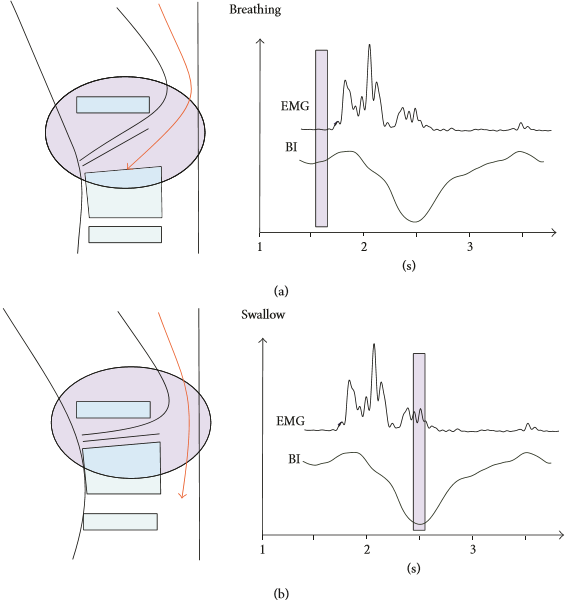
\includegraphics[width=9cm]
{Figure/EMGBIGraph}}
\caption{ggggggggg\cite{Bass1992Dysphagia:Management}}
\label{EMGBIGraph}
\end{figure}

\section{Formål}

Formålet med dette projekt er at udvikle et produkt, der består af et device, der kan måle pålidelige bioimpedans, samt kombinere bioimpedans måleren med en kommerciel EMG sensor for at kunne detektere synkefrekvensen på raske objekter, se figur \ref{KonceptuelDiagram}.


\begin{figure}[H]
\centering
{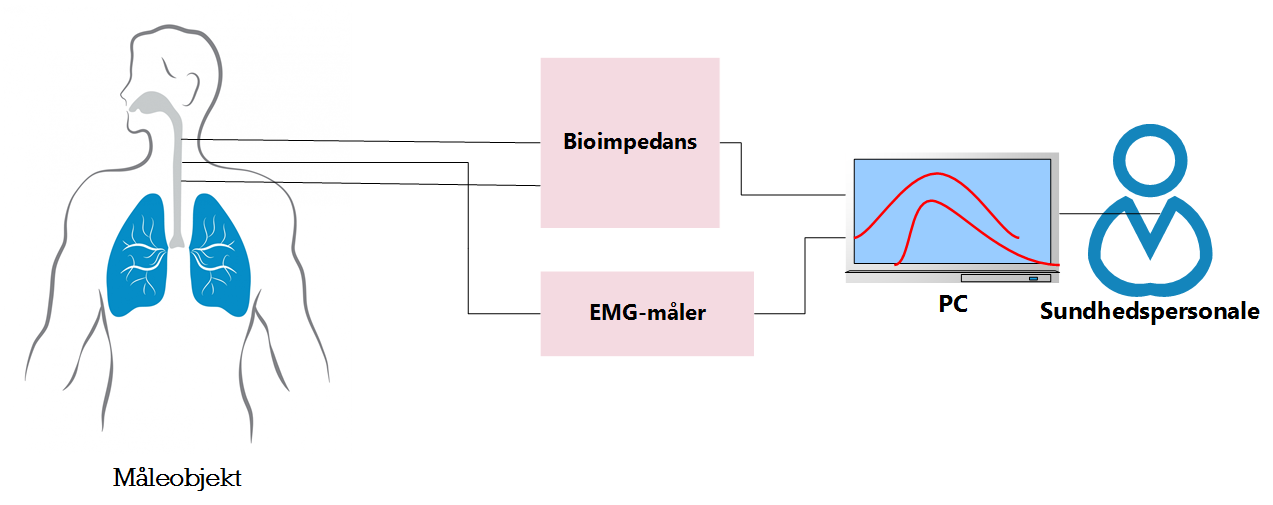
\includegraphics[width=11cm]
{Figure/KonceptuelDiagram}}
\caption{Viser det overordnet system som dette projekt vil realisere}
\label{KonceptuelDiagram}
\end{figure}

%\section{Problemformulering}